\documentclass{beamer}

%
% Common preamble for all three parts.
%

\usepackage[english]{babel}
\usepackage{amsmath}
\usepackage{color}
\usepackage{minted}
\usepackage{hyperref}
\usepackage{multicol}
\usepackage{tabularx}
\usepackage{tikz}

% only inline todonotes work
\usepackage{xkeyval}
\usepackage[textsize=small]{todonotes}
\presetkeys{todonotes}{inline}{}

\usetikzlibrary{shapes,arrows,positioning,shadows}

% no nav buttons
\usenavigationsymbolstemplate{}

\newcommand{\bftt}[1]{\textbf{\texttt{#1}}}
\newcommand{\comment}[1]{{\color[HTML]{008080}\textit{\textbf{\texttt{#1}}}}}
\newcommand{\cmd}[1]{{\color[HTML]{008000}\bftt{#1}}}
\newcommand{\bs}{\char`\\}
\newcommand{\cmdbs}[1]{\cmd{\bs#1}}
\newcommand{\lcb}{\char '173}
\newcommand{\rcb}{\char '175}
\newcommand{\cmdbegin}[1]{\cmdbs{begin\lcb}\bftt{#1}\cmd{\rcb}}
\newcommand{\cmdend}[1]{\cmdbs{end\lcb}\bftt{#1}\cmd{\rcb}}

\newcommand{\wllogo}{\textbf{Overleaf}}

% this is where the example source files are loaded from
% do not include a trailing slash
\newcommand{\fileuri}{https://raw.github.com/jdleesmiller/latex-course/master/en}

\newcommand{\wlserver}{https://www.overleaf.com}
\newcommand{\wlnewdoc}[1]{\wlserver/docs?snip\_uri=\fileuri/#1\&splash=none}

\def\tikzname{Ti\emph{k}Z}

% from http://tex.stackexchange.com/questions/5226/keyboard-font-for-latex
\newcommand*\keystroke[1]{%
  \tikz[baseline=(key.base)]
    \node[%
      draw,
      fill=white,
      drop shadow={shadow xshift=0.25ex,shadow yshift=-0.25ex,fill=black,opacity=0.75},
      rectangle,
      rounded corners=2pt,
      inner sep=1pt,
      line width=0.5pt,
      font=\scriptsize\sffamily
    ](key) {#1\strut}
  ;
}
\newcommand{\keystrokebftt}[1]{\keystroke{\bftt{#1}}}

% stolen from minted.dtx
\newenvironment{exampletwoup}
  {\VerbatimEnvironment
   \begin{VerbatimOut}{example.out}}
  {\end{VerbatimOut}
   \setlength{\parindent}{0pt}
   \fbox{\begin{tabular}{l|l}
   \begin{minipage}{0.55\linewidth}
     \inputminted[fontsize=\small,resetmargins]{latex}{example.out}
   \end{minipage} &
   \begin{minipage}{0.35\linewidth}
     \input{example.out}
   \end{minipage}
   \end{tabular}}}

\newenvironment{exampletwouptiny}
  {\VerbatimEnvironment
   \begin{VerbatimOut}{example.out}}
  {\end{VerbatimOut}
   \setlength{\parindent}{0pt}
   \fbox{\begin{tabular}{l|l}
   \begin{minipage}{0.55\linewidth}
     \inputminted[fontsize=\scriptsize,resetmargins]{latex}{example.out}
   \end{minipage} &
   \begin{minipage}{0.35\linewidth}
     \setlength{\parskip}{6pt plus 1pt minus 1pt}%
     \raggedright\scriptsize\input{example.out}
   \end{minipage}
   \end{tabular}}}

\newenvironment{exampletwouptinynoframe}
  {\VerbatimEnvironment
   \begin{VerbatimOut}{example.out}}
  {\end{VerbatimOut}
   \setlength{\parindent}{0pt}
   \begin{tabular}{l|l}
   \begin{minipage}{0.55\linewidth}
     \inputminted[fontsize=\scriptsize,resetmargins]{latex}{example.out}
   \end{minipage} &
   \begin{minipage}{0.35\linewidth}
     \setlength{\parskip}{6pt plus 1pt minus 1pt}%
     \raggedright\scriptsize\input{example.out}
   \end{minipage}
   \end{tabular}}

\title{An Interactive Introduction to \LaTeX}
\author{Dr John D. Lees-Miller}
\titlegraphic{%

\includegraphics[height=36pt]{Overleaf-logo-300dpi}\\[1em]

\includegraphics[height=24pt]{UoB-logo}
\qquad

\includegraphics[height=24pt]{setsquared_supported}
}


\subtitle{Part 1: The Basics}

\begin{document}

%%%%%%%%%%%%%%%%%%%%%%%%%%%%%%%%%%%%%%%%%%%%%%%%%%%%%%%%%%%%%%%%%%%%%%%%%%%%%%%
%%%%%%%%%%%%%%%%%%%%%%%%%%%%%%%%%%%%%%%%%%%%%%%%%%%%%%%%%%%%%%%%%%%%%%%%%%%%%%%
%%%%%%%%%%%%%%%%%%%%%%%%%%%%%%%%%%%%%%%%%%%%%%%%%%%%%%%%%%%%%%%%%%%%%%%%%%%%%%%
\begin{frame}
\titlepage
\end{frame}

%%%%%%%%%%%%%%%%%%%%%%%%%%%%%%%%%%%%%%%%%%%%%%%%%%%%%%%%%%%%%%%%%%%%%%%%%%%%%%%
%%%%%%%%%%%%%%%%%%%%%%%%%%%%%%%%%%%%%%%%%%%%%%%%%%%%%%%%%%%%%%%%%%%%%%%%%%%%%%%
%%%%%%%%%%%%%%%%%%%%%%%%%%%%%%%%%%%%%%%%%%%%%%%%%%%%%%%%%%%%%%%%%%%%%%%%%%%%%%%
\begin{frame}{Why \LaTeX{}?}
\begin{itemize}
\item It makes beautiful documents
\begin{itemize}
\item Especially mathematics
\end{itemize}
%
\item It was created by scientists, for scientists
\begin{itemize}
\item A large and active community
\end{itemize}
%
\item It is powerful --- you can extend it
\begin{itemize}
\item Packages for papers, presentations, spreadsheets, \ldots
\end{itemize}
\end{itemize}
\end{frame}

%%%%%%%%%%%%%%%%%%%%%%%%%%%%%%%%%%%%%%%%%%%%%%%%%%%%%%%%%%%%%%%%%%%%%%%%%%%%%%%
%%%%%%%%%%%%%%%%%%%%%%%%%%%%%%%%%%%%%%%%%%%%%%%%%%%%%%%%%%%%%%%%%%%%%%%%%%%%%%%
%%%%%%%%%%%%%%%%%%%%%%%%%%%%%%%%%%%%%%%%%%%%%%%%%%%%%%%%%%%%%%%%%%%%%%%%%%%%%%%
\begin{frame}[fragile]{How does it work?}
\begin{itemize}
\item You write your document in \texttt{plain text} with \cmd{commands} that
describe its structure and meaning.
\item The \texttt{latex} program processes your text and commands to produce a
beautifully formatted document.
\end{itemize}
\vskip 2ex
\begin{center}
\begin{minted}[frame=single]{latex}
The rain in Spain falls \emph{mainly} on the plain.
\end{minted}
\vskip 2ex
\tikz\node[single arrow,fill=gray,font=\ttfamily\bfseries,%
  rotate=270,xshift=-1em]{latex};
\vskip 2ex
\fbox{The rain in Spain falls \emph{mainly} on the plain.}
\end{center}
\end{frame}

%%%%%%%%%%%%%%%%%%%%%%%%%%%%%%%%%%%%%%%%%%%%%%%%%%%%%%%%%%%%%%%%%%%%%%%%%%%%%%%
%%%%%%%%%%%%%%%%%%%%%%%%%%%%%%%%%%%%%%%%%%%%%%%%%%%%%%%%%%%%%%%%%%%%%%%%%%%%%%%
%%%%%%%%%%%%%%%%%%%%%%%%%%%%%%%%%%%%%%%%%%%%%%%%%%%%%%%%%%%%%%%%%%%%%%%%%%%%%%%
\begin{frame}[fragile]{More examples of commands and their output\ldots}
\begin{exampletwoup}
\begin{itemize}
\item Tea
\item Milk
\item Biscuits
\end{itemize}
\end{exampletwoup}
\vskip 2ex
\begin{exampletwoup}
\begin{figure}
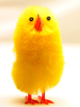
\includegraphics{chick}
\end{figure}
\end{exampletwoup}
\vskip 2ex
\begin{exampletwoup}
\begin{equation}
\alpha + \beta + 1
\end{equation}
\end{exampletwoup}

\tiny{Image from \url{http://www.andy-roberts.net/writing/latex/importing_images}}
\end{frame}

%%%%%%%%%%%%%%%%%%%%%%%%%%%%%%%%%%%%%%%%%%%%%%%%%%%%%%%%%%%%%%%%%%%%%%%%%%%%%%%
%%%%%%%%%%%%%%%%%%%%%%%%%%%%%%%%%%%%%%%%%%%%%%%%%%%%%%%%%%%%%%%%%%%%%%%%%%%%%%%
%%%%%%%%%%%%%%%%%%%%%%%%%%%%%%%%%%%%%%%%%%%%%%%%%%%%%%%%%%%%%%%%%%%%%%%%%%%%%%%
\begin{frame}[fragile]{Attitude adjustment}

\begin{itemize}
\item Use commands to describe `what it is', not `how it looks'.
\item Focus on your content.
\item Let \LaTeX{} do its job.
\end{itemize}
\end{frame}

%%%%%%%%%%%%%%%%%%%%%%%%%%%%%%%%%%%%%%%%%%%%%%%%%%%%%%%%%%%%%%%%%%%%%%%%%%%%%%%
%%%%%%%%%%%%%%%%%%%%%%%%%%%%%%%%%%%%%%%%%%%%%%%%%%%%%%%%%%%%%%%%%%%%%%%%%%%%%%%
%%%%%%%%%%%%%%%%%%%%%%%%%%%%%%%%%%%%%%%%%%%%%%%%%%%%%%%%%%%%%%%%%%%%%%%%%%%%%%%
\section{The Basics}

%%%%%%%%%%%%%%%%%%%%%%%%%%%%%%%%%%%%%%%%%%%%%%%%%%%%%%%%%%%%%%%%%%%%%%%%%%%%%%%
%%%%%%%%%%%%%%%%%%%%%%%%%%%%%%%%%%%%%%%%%%%%%%%%%%%%%%%%%%%%%%%%%%%%%%%%%%%%%%%
%%%%%%%%%%%%%%%%%%%%%%%%%%%%%%%%%%%%%%%%%%%%%%%%%%%%%%%%%%%%%%%%%%%%%%%%%%%%%%%
\subsection{Getting started}
\begin{frame}[fragile]{\insertsubsection}
\begin{itemize}
\item A minimal \LaTeX{} document:
\inputminted[frame=single]{latex}{basics.tex}
\item Commands start with a \emph{backslash} \keystrokebftt{\bs}.
\item Every document starts with a \cmdbs{documentclass} command.
\item The \emph{argument} in curly braces \keystrokebftt{\{} \keystrokebftt{\}} tells \LaTeX{} what kind of document we are creating: an \bftt{article}.
\item A percent sign \keystrokebftt{\%} starts a \emph{comment} --- \LaTeX{}
will ignore the rest of the line.
\end{itemize}
\end{frame}

%%%%%%%%%%%%%%%%%%%%%%%%%%%%%%%%%%%%%%%%%%%%%%%%%%%%%%%%%%%%%%%%%%%%%%%%%%%%%%%
%%%%%%%%%%%%%%%%%%%%%%%%%%%%%%%%%%%%%%%%%%%%%%%%%%%%%%%%%%%%%%%%%%%%%%%%%%%%%%%
%%%%%%%%%%%%%%%%%%%%%%%%%%%%%%%%%%%%%%%%%%%%%%%%%%%%%%%%%%%%%%%%%%%%%%%%%%%%%%%
\begin{frame}[fragile]{\insertsubsection{} with \wllogo}
\begin{itemize}
\item Overleaf is a website for writing documents in \LaTeX.
\item It `compiles' your \LaTeX{} automatically to show you the results.
\vskip 2em
\begin{center}
\fbox{\href{\wlnewdoc{basics.tex}}{%
Click here to open the example document in \wllogo{}}}
\\[1ex]\scriptsize{}
For best results, please use \href{http://www.google.com/chrome}{Google Chrome} or a recent \href{http://www.mozilla.org/en-US/firefox/new/}{FireFox}.
\end{center}
\vskip 2ex
\item As we go through the following slides, try out the examples by typing them
into the example document on Overleaf.
\item \textbf{No really, you should try them out as we go!}
\end{itemize}
\end{frame}

%%%%%%%%%%%%%%%%%%%%%%%%%%%%%%%%%%%%%%%%%%%%%%%%%%%%%%%%%%%%%%%%%%%%%%%%%%%%%%%
%%%%%%%%%%%%%%%%%%%%%%%%%%%%%%%%%%%%%%%%%%%%%%%%%%%%%%%%%%%%%%%%%%%%%%%%%%%%%%%
%%%%%%%%%%%%%%%%%%%%%%%%%%%%%%%%%%%%%%%%%%%%%%%%%%%%%%%%%%%%%%%%%%%%%%%%%%%%%%%
\subsection{Typesetting Text}
\begin{frame}[fragile]{\insertsubsection{}}
\small
\begin{itemize}
\item Type your text between \cmdbegin{document} and \cmdend{document}.
\item For the most part, you can just type your text normally.
\begin{exampletwouptiny}
Words are separated by one or more
spaces.

Paragraphs are separated by one
or more blank lines.
\end{exampletwouptiny}
\item Space in the source file is collapsed in the output.
\begin{exampletwouptiny}
The   rain       in Spain
falls mainly on the plain.
\end{exampletwouptiny}
\end{itemize}
\end{frame}

%%%%%%%%%%%%%%%%%%%%%%%%%%%%%%%%%%%%%%%%%%%%%%%%%%%%%%%%%%%%%%%%%%%%%%%%%%%%%%%
%%%%%%%%%%%%%%%%%%%%%%%%%%%%%%%%%%%%%%%%%%%%%%%%%%%%%%%%%%%%%%%%%%%%%%%%%%%%%%%
%%%%%%%%%%%%%%%%%%%%%%%%%%%%%%%%%%%%%%%%%%%%%%%%%%%%%%%%%%%%%%%%%%%%%%%%%%%%%%%
\begin{frame}[fragile]{\insertsubsection{}: Caveats}
\small
\begin{itemize}
\item Quotation marks are a bit tricky: use a backtick \keystroke{\`{}} on the left and an apostrophe \keystroke{\'{}} on the right.
\begin{exampletwouptiny}
Single quotes: `text'.

Double quotes: ``text''.
\end{exampletwouptiny}

\item Some common characters have special meanings in \LaTeX:\\[1ex]
\begin{tabular}{cl}
\keystrokebftt{\%} & percent sign              \\
\keystrokebftt{\#} & hash (pound / sharp) sign \\
\keystrokebftt{\&} & ampersand                 \\
\keystrokebftt{\$} & dollar sign               \\
\end{tabular}
\item If you just type these, you'll get an error. If you want one to appear in
the output, you have to \emph{escape} it by preceding it with a backslash.
\begin{exampletwoup}
\$\%\&\#!
\end{exampletwoup}
\end{itemize}
\end{frame}

%%%%%%%%%%%%%%%%%%%%%%%%%%%%%%%%%%%%%%%%%%%%%%%%%%%%%%%%%%%%%%%%%%%%%%%%%%%%%%%
%%%%%%%%%%%%%%%%%%%%%%%%%%%%%%%%%%%%%%%%%%%%%%%%%%%%%%%%%%%%%%%%%%%%%%%%%%%%%%%
%%%%%%%%%%%%%%%%%%%%%%%%%%%%%%%%%%%%%%%%%%%%%%%%%%%%%%%%%%%%%%%%%%%%%%%%%%%%%%%
\begin{frame}[fragile]{Handling Errors}
\begin{itemize}
\item \LaTeX{} can get confused when it is trying to compile your document. If
it does, it stops with an error, which you must fix before it will produce
any output.
\item For example, if you misspell \cmdbs{emph} as \cmdbs{meph}, \LaTeX{} will
stop with an ``undefined control sequence'' error, because ``meph'' is not
one of the commands it knows.
\end{itemize}
\begin{block}{Advice on Errors}
\begin{enumerate}
\item Don't panic! Errors happen.
\item Fix them as soon as they arise --- if what you just typed caused an error,
you can start your debugging there.
\item If there are multiple errors, start with the first one --- the cause may
even be above it.
\end{enumerate}
\end{block}
\end{frame}

%%%%%%%%%%%%%%%%%%%%%%%%%%%%%%%%%%%%%%%%%%%%%%%%%%%%%%%%%%%%%%%%%%%%%%%%%%%%%%%
%%%%%%%%%%%%%%%%%%%%%%%%%%%%%%%%%%%%%%%%%%%%%%%%%%%%%%%%%%%%%%%%%%%%%%%%%%%%%%%
%%%%%%%%%%%%%%%%%%%%%%%%%%%%%%%%%%%%%%%%%%%%%%%%%%%%%%%%%%%%%%%%%%%%%%%%%%%%%%%
\begin{frame}[fragile]{Typesetting Exercise 1}

\begin{block}{Typeset this in \LaTeX:
\footnote{\url{http://en.wikipedia.org/wiki/Economy_of_the_United_States}}}
In March 2006, Congress raised that ceiling an additional \$0.79 trillion to
\$8.97 trillion, which is approximately 68\% of GDP. As of October 4, 2008, the
``Emergency Economic Stabilization Act of 2008'' raised the current debt ceiling
to \$11.3 trillion.
\end{block}
\vskip 2ex
\begin{center}
\fbox{\href{\wlnewdoc{basics-exercise-1.tex}}{%
Click to open this exercise in \wllogo{}}}
\end{center}

\begin{itemize}
\item Hint: watch out for characters with special meanings!
\item Once you've tried,
\fbox{\href{\wlnewdoc{basics-exercise-1-solution.tex}}{%
click here to see my solution}}.
\end{itemize}
\end{frame}

%%%%%%%%%%%%%%%%%%%%%%%%%%%%%%%%%%%%%%%%%%%%%%%%%%%%%%%%%%%%%%%%%%%%%%%%%%%%%%%
%%%%%%%%%%%%%%%%%%%%%%%%%%%%%%%%%%%%%%%%%%%%%%%%%%%%%%%%%%%%%%%%%%%%%%%%%%%%%%%
%%%%%%%%%%%%%%%%%%%%%%%%%%%%%%%%%%%%%%%%%%%%%%%%%%%%%%%%%%%%%%%%%%%%%%%%%%%%%%%
\subsection{Typesetting Mathematics}
\begin{frame}[fragile]{\insertsubsection{}: Dollar Signs}
\begin{itemize}
\item Why are dollar signs \keystrokebftt{\$} special? We use them to mark mathematics in text.\\[1ex]
\begin{exampletwouptiny}
% not so good:
Let a and b be distinct positive
integers, and let c = a - b + 1.

% much better:
Let $a$ and $b$ be distinct positive
integers, and let $c = a - b + 1$.
\end{exampletwouptiny}
\item Always use dollar signs in pairs --- one to begin the mathematics, and one
to end it.
\item \LaTeX{} handles spacing automatically; it ignores your spaces.
\begin{exampletwouptiny}
Let $y=mx+b$ be \ldots

Let $y = m x + b$ be \ldots
\end{exampletwouptiny}
\end{itemize}
\end{frame}

%%%%%%%%%%%%%%%%%%%%%%%%%%%%%%%%%%%%%%%%%%%%%%%%%%%%%%%%%%%%%%%%%%%%%%%%%%%%%%%
%%%%%%%%%%%%%%%%%%%%%%%%%%%%%%%%%%%%%%%%%%%%%%%%%%%%%%%%%%%%%%%%%%%%%%%%%%%%%%%
%%%%%%%%%%%%%%%%%%%%%%%%%%%%%%%%%%%%%%%%%%%%%%%%%%%%%%%%%%%%%%%%%%%%%%%%%%%%%%%
\begin{frame}[fragile]{\insertsubsection{}: Notation}
\begin{itemize}
\item Use caret \keystrokebftt{\^} for superscripts and underscore \keystrokebftt{\_} for subscripts.
\begin{exampletwouptiny}
$y = c_2 x^2 + c_1 x + c_0$
\end{exampletwouptiny}
\vskip 2ex

\item Use curly braces \keystrokebftt{\{} \keystrokebftt{\}} to group
superscripts and subscripts.
\begin{exampletwouptiny}
$F_n = F_n-1 + F_n-2$     % oops!

$F_n = F_{n-1} + F_{n-2}$ % ok!
\end{exampletwouptiny}
\vskip 2ex

\item There are commands for Greek letters and common notation.
\begin{exampletwouptiny}
$\mu = A e^{Q/RT}$

$\Omega = \sum_{k=1}^{n} \omega_k$
\end{exampletwouptiny}
\end{itemize}
\end{frame}

%%%%%%%%%%%%%%%%%%%%%%%%%%%%%%%%%%%%%%%%%%%%%%%%%%%%%%%%%%%%%%%%%%%%%%%%%%%%%%%
%%%%%%%%%%%%%%%%%%%%%%%%%%%%%%%%%%%%%%%%%%%%%%%%%%%%%%%%%%%%%%%%%%%%%%%%%%%%%%%
%%%%%%%%%%%%%%%%%%%%%%%%%%%%%%%%%%%%%%%%%%%%%%%%%%%%%%%%%%%%%%%%%%%%%%%%%%%%%%%
\begin{frame}[fragile]{\insertsubsection{}: Displayed Equations}
\begin{itemize}
\item If it's big and scary, \emph{display} it on its own line using
\cmdbegin{equation} and \cmdend{equation}.\\[2ex]
\begin{exampletwouptiny}
The roots of a quadratic equation
are given by
\begin{equation}
x = \frac{-b \pm \sqrt{b^2 - 4ac}}
         {2a}
\end{equation}
where $a$, $b$ and $c$ are \ldots
\end{exampletwouptiny}
\vskip 1em
{\scriptsize Caution: \LaTeX{} mostly ignores your spaces in mathematics, but it
can't handle blank lines in equations --- don't put blank lines in your
mathematics.}
\end{itemize}
\end{frame}

%%%%%%%%%%%%%%%%%%%%%%%%%%%%%%%%%%%%%%%%%%%%%%%%%%%%%%%%%%%%%%%%%%%%%%%%%%%%%%%
%%%%%%%%%%%%%%%%%%%%%%%%%%%%%%%%%%%%%%%%%%%%%%%%%%%%%%%%%%%%%%%%%%%%%%%%%%%%%%%
%%%%%%%%%%%%%%%%%%%%%%%%%%%%%%%%%%%%%%%%%%%%%%%%%%%%%%%%%%%%%%%%%%%%%%%%%%%%%%%
\begin{frame}[fragile]{Interlude: Environments}
\begin{itemize}
\item \bftt{equation} is an \emph{environment} --- a context.
\item A command can produce different output in different contexts.
\begin{exampletwouptiny}
We can write
$ \Omega = \sum_{k=1}^{n} \omega_k $
in text, or we can write
\begin{equation}
  \Omega = \sum_{k=1}^{n} \omega_k
\end{equation}
to display it.
\end{exampletwouptiny}
\vskip 2ex
\item Note how the $\Sigma$ is bigger in the \bftt{equation} environment, and
how the subscripts and superscripts change position, even though we used the
same commands.
\vskip 1em
{\scriptsize In fact, we could have written \bftt{\$...\$} as
\cmdbegin{math}\bftt{...}\cmdend{math}.}
\end{itemize}
\end{frame}

%%%%%%%%%%%%%%%%%%%%%%%%%%%%%%%%%%%%%%%%%%%%%%%%%%%%%%%%%%%%%%%%%%%%%%%%%%%%%%%
%%%%%%%%%%%%%%%%%%%%%%%%%%%%%%%%%%%%%%%%%%%%%%%%%%%%%%%%%%%%%%%%%%%%%%%%%%%%%%%
%%%%%%%%%%%%%%%%%%%%%%%%%%%%%%%%%%%%%%%%%%%%%%%%%%%%%%%%%%%%%%%%%%%%%%%%%%%%%%%
\begin{frame}[fragile]{Interlude: Environments}
\begin{itemize}
\item The \cmdbs{begin} and \cmdbs{end} commands are used to create many
different environments.
\vskip 2ex

\item The \bftt{itemize} and \bftt{enumerate} environments generate lists.
\begin{exampletwouptiny}
\begin{itemize} % for bullet points
\item Biscuits
\item Tea
\end{itemize}

\begin{enumerate} % for numbers
\item Biscuits
\item Tea
\end{enumerate}
\end{exampletwouptiny}
\end{itemize}
\end{frame}

%%%%%%%%%%%%%%%%%%%%%%%%%%%%%%%%%%%%%%%%%%%%%%%%%%%%%%%%%%%%%%%%%%%%%%%%%%%%%%%
%%%%%%%%%%%%%%%%%%%%%%%%%%%%%%%%%%%%%%%%%%%%%%%%%%%%%%%%%%%%%%%%%%%%%%%%%%%%%%%
%%%%%%%%%%%%%%%%%%%%%%%%%%%%%%%%%%%%%%%%%%%%%%%%%%%%%%%%%%%%%%%%%%%%%%%%%%%%%%%
\begin{frame}[fragile]{Interlude: Packages}

\begin{itemize}
\item All of the commands and environments we've used so far are built into
\LaTeX.

\item \emph{Packages} are libraries of extra commands and environments. There
are thousands of freely available packages.

\item We have to load each of the packages we want to use with a
\cmdbs{usepackage} command in the \emph{preamble}.

\item Example: \bftt{amsmath} from the American Mathematical Society.
\begin{minted}[fontsize=\small,frame=single]{latex}
\documentclass{article}
\usepackage{amsmath} % preamble
\begin{document}
% now we can use commands from amsmath here...
\end{document}
\end{minted}
\end{itemize}
\end{frame}

%%%%%%%%%%%%%%%%%%%%%%%%%%%%%%%%%%%%%%%%%%%%%%%%%%%%%%%%%%%%%%%%%%%%%%%%%%%%%%%
%%%%%%%%%%%%%%%%%%%%%%%%%%%%%%%%%%%%%%%%%%%%%%%%%%%%%%%%%%%%%%%%%%%%%%%%%%%%%%%
%%%%%%%%%%%%%%%%%%%%%%%%%%%%%%%%%%%%%%%%%%%%%%%%%%%%%%%%%%%%%%%%%%%%%%%%%%%%%%%
\begin{frame}[fragile]{\insertsubsection{}: Examples with \bftt{amsmath}}
\begin{itemize}
\item Use \bftt{equation*} (``equation-star'') for unnumbered equations.
\begin{exampletwouptiny}
\begin{equation*}
  \Omega = \sum_{k=1}^{n} \omega_k
\end{equation*}
\end{exampletwouptiny}
\item \LaTeX{} treats adjacent letters as variables multiplied together, which
is not always what you want. \bftt{amsmath} defines commands for many common
mathematical operators.
\begin{exampletwouptiny}
\begin{equation*} % bad!
 min_{x,y} (1-x)^2 + 100(y-x^2)^2
\end{equation*}
\begin{equation*} % good!
\min_{x,y}{(1-x)^2 + 100(y-x^2)^2}
\end{equation*}
\end{exampletwouptiny}
\item You can use \cmdbs{operatorname} for others.
\begin{exampletwouptiny}
\begin{equation*}
\beta_i =
\frac{\operatorname{Cov}(R_i, R_m)}
     {\operatorname{Var}(R_m)}
\end{equation*}
\end{exampletwouptiny}
\end{itemize}
\end{frame}

%%%%%%%%%%%%%%%%%%%%%%%%%%%%%%%%%%%%%%%%%%%%%%%%%%%%%%%%%%%%%%%%%%%%%%%%%%%%%%%
%%%%%%%%%%%%%%%%%%%%%%%%%%%%%%%%%%%%%%%%%%%%%%%%%%%%%%%%%%%%%%%%%%%%%%%%%%%%%%%
%%%%%%%%%%%%%%%%%%%%%%%%%%%%%%%%%%%%%%%%%%%%%%%%%%%%%%%%%%%%%%%%%%%%%%%%%%%%%%%
\begin{frame}[fragile]{\insertsubsection{}: Examples with \bftt{amsmath}}
\begin{itemize}{\small
\item Align a sequence of equations at the equals sign
\begin{align*}
(x+1)^3 &= (x+1)(x+1)(x+1) \\
        &= (x+1)(x^2 + 2x + 1) \\
        &= x^3 + 3x^2 + 3x + 1
\end{align*}
with the \bftt{align*} environment.

% for whatever reason, this doesn't play well with the twoup environment
\begin{minted}[fontsize=\small,frame=single]{latex}
\begin{align*}
(x+1)^3 &= (x+1)(x+1)(x+1) \\
        &= (x+1)(x^2 + 2x + 1) \\
        &= x^3 + 3x^2 + 3x + 1
\end{align*}
\end{minted}
\item An ampersand \keystrokebftt{\&} separates the left column (before the
$=$) from the right column (after the $=$).
\item A double backslash \keystrokebftt{\bs}\keystrokebftt{\bs} starts a new
line.
}\end{itemize}
\end{frame}


%%%%%%%%%%%%%%%%%%%%%%%%%%%%%%%%%%%%%%%%%%%%%%%%%%%%%%%%%%%%%%%%%%%%%%%%%%%%%%%
%%%%%%%%%%%%%%%%%%%%%%%%%%%%%%%%%%%%%%%%%%%%%%%%%%%%%%%%%%%%%%%%%%%%%%%%%%%%%%%
%%%%%%%%%%%%%%%%%%%%%%%%%%%%%%%%%%%%%%%%%%%%%%%%%%%%%%%%%%%%%%%%%%%%%%%%%%%%%%%
\begin{frame}[fragile]{Typesetting Exercise 2}

\begin{block}{Typeset this in \LaTeX:}
Let $X_1, X_2, \ldots, X_n$ be a sequence of independent and identically
distributed random variables with $\operatorname{E}[X_i] = \mu$ and
$\operatorname{Var}[X_i] = \sigma^2 < \infty$, and let
\begin{equation*}
S_n = \frac{1}{n}\sum_{i}^{n} X_i
\end{equation*}
denote their mean. Then as $n$ approaches infinity, the random variables
$\sqrt{n}(S_n - \mu)$ converge in distribution to a normal $N(0, \sigma^2)$.
\end{block}
\vskip 2ex
\begin{center}
\fbox{\href{\wlnewdoc{basics-exercise-2.tex}}{%
Click to open this exercise in \wllogo{}}}
\end{center}
\begin{itemize}
\item Hint: the command for $\infty$ is \cmdbs{infty}.
\item Once you've tried,
\fbox{\href{\wlnewdoc{basics-exercise-2-solution.tex}}{%
click here to see my solution}}.
\end{itemize}
\end{frame}

%%%%%%%%%%%%%%%%%%%%%%%%%%%%%%%%%%%%%%%%%%%%%%%%%%%%%%%%%%%%%%%%%%%%%%%%%%%%%%%
%%%%%%%%%%%%%%%%%%%%%%%%%%%%%%%%%%%%%%%%%%%%%%%%%%%%%%%%%%%%%%%%%%%%%%%%%%%%%%%
%%%%%%%%%%%%%%%%%%%%%%%%%%%%%%%%%%%%%%%%%%%%%%%%%%%%%%%%%%%%%%%%%%%%%%%%%%%%%%%
\begin{frame}{End of Part 1}
\begin{itemize}
\item Congrats! You've already learned how to \ldots
\begin{itemize}
\item Typeset text in \LaTeX.
\item Use lots of different commands.
\item Handle errors when they arise.
\item Typeset some beautiful mathematics.
\item Use several different environments.
\item Load packages.
\end{itemize}
\item That's amazing!
\item In Part 2, we'll see how to use \LaTeX{} to write structured documents
with sections, cross references, figures, tables and bibliographies. See you
then!
\end{itemize}
\end{frame}

\end{document}
